

\chapter{Markov-Ketten, Hidden Markov Modelle}
Eine Markov-Kette ist ein stochastischer Prozess, der durch Zustände und Über-gangswahrscheinlichkeiten beschrieben wird.
\begin{figure}[htbp]
	\centering
		\begin{tikzpicture}[node distance=2cm]
			\node[state] (z_0)                {$z_0$};
			\node[state] (z_1) [right of=z_0] {$z_1$};
			\path[->] 
				(z_0) 
					edge [loop above] node {0,3} ()
					edge [bend left, above] node {0,7} (z_1)
				(z_1) 
					edge [loop above] node {0,6} ()
					edge [bend left, below] node {0,4} (z_0);
		\end{tikzpicture}
\end{figure}

Damit lassen sich modellieren:
\begin{itemize}
	\item Texte in natürlicher Sprache (Zustände: Buchstaben)
	\item DNA-Sequenzen (Zustände: A,C,G,T)
	\item Navigation im Internet (Zustände: Webseiten)
\end{itemize}


\section{Hidden Markov Model (HMM)}
\begin{shaded}
  \noindent
  \textbf{Def.:} Ein HHM ist eine Markov-Kette, die in jeden Zustand z ein Zeichen a ausgibt mit der Wahrscheinlichkeit \(q_z(a)\).
\end{shaded}
\begin{figure}[htbp]
	\centering
	\begin{tikzpicture}[node distance=4cm]
		\node[state] (z_0)                {\(z_0\)};
		\node[state] (z_1) [right=4cm of z_0] {\(z_1\)};
		\node[emission] (a) [below of=z_0] {a};
		\node[emission] (b) [below of=z_1] {b};
		\path[->] 
			(z_0) 
				edge [loop above] node {0,5} ()
				edge [bend left, above] node {0,5} (z_1)
				edge [left] node {0,6} (a)
				edge [left] node {0,4} (b)
			(z_1) 
				edge [loop above] node {0,9} ()
				edge [ above] node {0,1} (z_0)
				edge [right] node {0,9} (b)
				edge [right] node {0,1} (a);
	\end{tikzpicture}
\end{figure}
Beobachtet werden nur die vom HMM ausgegebenen Zeichen.
Unbekannt ist die Zustandsfolge.
Mit HMM können modelliert werden z.B.:
\begin{itemize}
	\item Codierende Regionen in DNA\\
		Zustände: A,C,T,G in codierenden und nicht codierenden Regionen\\
		Ausgegebene Zeichen: Jeweils A,C,T,G
	\item Nachrichtenübertragung\\
		Markov-Kette, die Texte modelliert\\
		In einem Zustand z wird das Zeichen z ausgegeben mit großer Wahrscheinlichkeit (z.B. 0,95), andere Zeichen mit geringer W'keit.
	\item Spracherkennung\\
		Vorgehen: Audio-Signal $\to$ FFT $\to$ Phoneme $\to$ Wort\\
		Zustände: Phoneme, die der Sprecher gesprochen hat.\\
		Ausgegebenen Zeichen: Phoneme, die das System erkannt hat oder das vom System erkannte Wort.
\end{itemize}

\subsubsection{Fragestellung}
Gegeben ist eine Folge von Ausgangszeichen eines HMM, welches ist die wahrscheinlichste Folge von Zuständen, die das HMM durchlaufen hat?
\subsubsection{Mathematische Behandlung}
Sei \(Z_k\) eine Zufallsvariable, die den Zustand des HMM im Schritt \(k\) angibt.
Aus \(Z_1\) ergibt sich die Startverteilung \[\pi_k=P(Z_1=k)\] der Markov-Kette.

Da \(Z_{k+1}\) nur von \(Z_k\) abhängt, folgt:
\begin{eqnarray*}
    &&P(\underbrace{Z_{k+1}}_{\text{Zufallsvariable}}=\underbrace{z_{k+1}}_{\text{Zustand}}|Z_k=z_k,\dots,Z_1=z_1)\\
	&=& P(Z_{k+1}=z_{k+1}|Z_k=z_k)\\
	&=:& p(z_k,z_{k+1})
\end{eqnarray*}
Sei \(A_k\) die Zufallsvariable, die das in Schritt \(k\) ausgegebene Zeichen angibt.
\(A_k\) hängt nur von \(Z_k\) ab:
\[P(A_k=a|Z_k=z_k,\dots,Z_1=z_1) = P(A_k=a|Z_k=z_k) =: q_{z_k}(a)\]
Die charakteristischen Größen eines HMM sind damit $\pi_k,\; p(z,z'),\; q_z(a)$.

Für eine Folge \(a_1,\dots,a_n\) von beobachteten Zeichen suchen wir eine Folge \(z_1,\dots,z_n\) von Zuständen, so dass
\[P(Z_1=z_1,\dots,Z_n=z_n|A_1=a_1,\dots,A_n=a_n)\]
maximal ist.
Da in
\begin{eqnarray*}
    \frac{P(Z_1=z_1, \dots, Z_n=z_n,\; A_1 = a_1, \dots, A_n=a_n)}{P(A_1=a_1, \dots, A_n=a_n)} \\
\end{eqnarray*}
der Nenner unabhängig von der Lösung ist, maximieren wir den Zähler.
%\begin{eqnarray*}
	%&&P(Z_1=z_1, \dots, Z_n=z_n | A_1=a_1, \dots A_n=a_n)\\
	%&=& \frac{P(Z_1=z_1, \dots, Z_n=z_n) \cap P(A_1 = a_1, \dots, A_n=a_n)}{P(A_1=a_1, \dots, A_n=a_n)} \\
	%&=& \frac{P(Z_1=z_1, \dots, Z_n=z_n, A_1 = a_1, \dots, A_n=a_n)}{P(A_1=a_1, \dots, A_n=a_n)}
%\end{eqnarray*}
%und der Nenner unabhängig von der Lösung ist (da er der Beobachtung entspricht), maximieren wir den Zähler.

Sei
\begin{eqnarray*}
	t(z_n,n) &=& P(Z_1=z_1, \dots, Z_n=z_n, A_1=a_1, \dots, A_n=a_n)\\
		&=& P(A_n=a_n|Z_1=z_1, \dots, Z_n=z_n, A_1=a_1, \dots, A_{n-1} = a_{n-1}) \cdot \\
		&& P(Z_1=z_1, \dots, Z_n=z_n, A_1=a_1, \dots, A_{n-1}=a_{n-1})\\
		&=& P(A_n=a_n|Z_n=z_n) \cdot \\
		&& P(Z_1=z_1, \dots, Z_n=z_n, A_1=a_1, \dots, A_{n-1}=a_{n-1})\\
		&=& q_{z_n}(a_n) \cdot\\
		&& P(Z_n=z_n|Z_1=z_1, \dots, Z_{n-1}=z_{n-1}, A_1=a_1, \dots, A_{n-1}=a_{n-1}) \cdot\\
		&& P(Z_1=z_1,\dots, Z_{n-1}=z_{n-1}, A_1=a_1, \dots, A_{n-1}=a_{n-1})\\
		&=& q_{z_n}(a_n) \cdot P(Z_n=z_n|Z_{n-1}=z_{n-1}) \cdot \\
		&& P(Z_1=z_1, \dots, Z_{n-1}=z_{n-1}, A_1=a_1, \dots, A_{n-1}=a_{n-1})\\
		&=& q_{z_n}(a_n) \cdot p(z_{n-1},z_n) \cdot t(z_{n-1},n-1)
\end{eqnarray*}



\section{Viterbi-Algorithmus}
Der Viterbi-Algorithmus ist ein Algorithmus der dynamischen Programmierung zur Bestimmung der wahrscheinlichsten Sequenz
von verborgenen Zuständen bei einem gegebenen Hidden Markov Model (HMM) und einer beobachteten Sequenz von Symbolen.
Diese Zustandssequenz wird auch als Viterbi-Pfad bezeichnet.
\begin{align*}
    t(Z,n) =
    \begin{cases}
        q_Z(a_1) \cdot \pi_Z 								& \text{für } n=1\\
        q_Z(a_n) \cdot \max_{z'} \left(p(z',z) \cdot t(z',n-1)\right) & \text{für } n>1\\
    \end{cases}
\end{align*}
Die Laufzeit beträgt \(\underbrace{\mathcal{O}(|Z| \cdot n)}_{\text{Größe der
            Tabelle}} \cdot \underbrace{\mathcal{O}(|Z|)}_{\text{Aufwand pro
            Zelle}} = \mathcal{O}(|Z|^2 \cdot n)\)

\begin{figure}[htbp]
	\centering
	\begin{tikzpicture}[node distance=1.5cm]
		\node[state] (z)                  {z};
		\node[state] (z') [left=1.5cm of z]     {z'};
		\node[state] (e1) [above of=z']  {};
		\node[state] (e2) [below of=z'] {};
        \node (a) [below=.5cm of e2] {\(\underbrace{a_1\; \dots\; a_{k-1}}_{t(z',k-1)}\)};
		\node[emission] (ak) [below of=z] {$a_k$};
		\path[->] 
			(e1) edge (z)
			(e2) edge (z)
			(z') edge [above] node {P(z',z)} (z)
			(z)	 edge [right] node {\(q_z(a_k)\)} (ak);
	\end{tikzpicture}
    \caption{Verdeutlichung des Viterbi-Algorithmusses.}\label{fig:viterbi}
\end{figure}
Um die numerische Stabilität des Verfahrens zu erhöhen, ist es Vorteilhaft, mit den Logarithmen zu rechnen.

\subsubsection{Beispiel}
Gegeben sei das folgende HMM-Model (\cref{fig:hmmbsp}) mit der Folge ``k z z k k z k k k k k k''
(mit k=Kopf, z=Zahl).
Berechnen Sie die wahrscheinlichste Zustandsfolge die diese Folge erzeugt hat
\begin{figure}[htbp]
	\centering
	\begin{tikzpicture}[node distance=2cm]
		\node[state] (z0)                 {z0};
		\node[state] (z1) [right of=z0]   {z1};
		\node[emission] (k) [below of=z0] {k};
		\node[emission] (z) [below of=z1] {z};
		\path[->] 
			(0.9,1.5) 
				edge [left] node {0,9} (z0)
				edge [right] node {0,1} (z1)
			(z0) 
				edge [loop left] node {0,9} ()
				edge [bend left, above] node {0,1} (z1)
				edge [left] node {0,5} (k)
				edge [left] node {0,5} (z)
			(z1) 
				edge [loop right] node {0,9} ()
				edge [bend left, above] node {0,1} (z0)
				edge [right] node {0,1} (z)
				edge [right] node {0,9} (k);
	\end{tikzpicture}
    \caption{HMM für Beispiel X.}\label{fig:hmmbsp}
\end{figure}

\begin{center}
\begin{tabular}{cccc}
				& \(z_{0}\) & \(z_{1}\) & \\ \hline
\(t(z',1)\)= k	& \(0,5\cdot0,9 = 0,4500;\) & \(0,9\cdot0,1 = 0,0900\) & \(z_{0}\) \\ \hline
\(t(z',2)\)= z	& \(	\begin{array} {r@{}l@{}}
							0,5\cdot\max\{	& 0,9\cdot0,45; \\
											& 0,1\cdot0,09\}\\
										   =& 0,2025
					\end{array}
					\)
				&  \(	\begin{array} {r@{}l@{}}
							0,1\cdot\max\{	& 0,9\cdot0,09; \\
											& 0,1\cdot0,45\}\\
										   =& 0,0081
					\end{array}
					\) & \(z_{0}\) \\ \hline
\(t(z',3)\)= z	& \(	\begin{array} {r@{}l@{}}
							0,5\cdot\max\{	& 0,9\cdot0,2; \\
											& 0,1\cdot0,0081\}\\
										   =& 0,091125
					\end{array}
					\)
				&   \(	\begin{array} {r@{}l@{}}
							0,1\cdot\max\{	& 0,9\cdot0,008; \\
											& 0,1\cdot0,2\}\\
										   =& 0,002025
					\end{array}
					\) & \(z_{0}\)\\ \hline
\(t(z',4)\)= k	& \(	\begin{array} {r@{}l@{}}
							0,5\cdot\max\{	& 0,9\cdot0,09; \\
											& 0,1\cdot0,002\}\\
										   =& 0,04100625
					\end{array}
					\)
				&   \(	\begin{array} {r@{}l@{}}
							0,9\cdot\max\{	& 0,9\cdot0,002; \\
											& 0,1\cdot0,09\}\\
										   =& 0,00820125
					\end{array}
					\) & \(z_{0}\)\\ \hline
\(t(z',5)\)= k	& \(	\begin{array} {r@{}l@{}}
							0,5\cdot\max\{	& 0,9\cdot0,041; \\
											& 0,1\cdot0,0082\}\\
										   =& 0,0184528125
					\end{array}
					\)
				&   \(	\begin{array} {r@{}l@{}}
							0,9\cdot\max\{	& 0,9\cdot0,0082; \\
											& 0,1\cdot0,041\}\\
										   =& 0,0066430125
					\end{array}
					\) & \(z_{0}\)\\ \hline
\(t(z',6)\)= z	& \(	\begin{array} {r@{}l@{}}
							0,5\cdot\max\{	& 0,9\cdot0,018; \\
											& 0,1\cdot0,007\}\\
										   =& 0,0083037656
					\end{array}
					\)
				&   \(	\begin{array} {r@{}l@{}}
							0,1\cdot\max\{	& 0,9\cdot0,007; \\
											& 0,1\cdot0,018\}\\
										   =& 0,00063
					\end{array}
					\) & \(z_{0}\)\\ \hline
\(t(z',7)\)= k	& \(	\begin{array} {r@{}l@{}}
							0,5\cdot\max\{	& 0,9\cdot0,0081; \\
											& 0,1\cdot0,00063\}\\
										   =& 0,0037366945
					\end{array}
					\)
				&   \(	\begin{array} {r@{}l@{}}
							0,9\cdot\max\{	& 0,9\cdot0,00063; \\
											& 0,1\cdot0,0083\}\\
										   =& 0,0007473389
					\end{array}
					\) & \(z_{1}\)\\ \hline
\(t(z',8)\)= k	& \(	\begin{array} {r@{}l@{}}
							0,5\cdot\max\{	& 0,9\cdot0,0037; \\
											& 0,1\cdot0,00075\}\\
										   =& 0,0016815254
					\end{array}
					\)
				&   \(	\begin{array} {r@{}l@{}}
							0,9\cdot\max\{	& 0,9\cdot0,00075; \\
											& 0,1\cdot0,0037\}\\
										   =& 0,0006053445
					\end{array}
					\) & \(z_{1}\)\\ \hline
\(t(z',9)\)= k	& \(	\begin{array} {r@{}l@{}}
							0,5\cdot\max\{	& 0,9\cdot0,00162; \\
											& 0,1\cdot0,00059\}\\
										   =& 0,0007566806
					\end{array}
					\)
				&   \(	\begin{array} {r@{}l@{}}
							0,9\cdot\max\{	& 0,9\cdot0,0006; \\
											& 0,1\cdot0,00162\}\\
										   =& 0,0004903291
					\end{array}
					\) & \(z_{1}\)\\ \hline
\(t(z',10)\)= k	& \(	\begin{array} {r@{}l@{}}
							0,5\cdot\max\{	& 0,9\cdot0,000729; \\
											& 0,1\cdot0,0004779\}\\
										   =& 0,000328
					\end{array}
					\)
				&   \(	\begin{array} {r@{}l@{}}
							0,9\cdot\max\{	& 0,9\cdot0,0004779; \\
											& 0,1\cdot0,000729\}\\
										   =& 0,0003971665
					\end{array}
					\) & \(z_{1}\)\\ \hline
\(t(z',11)\)= k	& \(	\begin{array} {r@{}l@{}}
							0,5\cdot\max\{	& 0,9\cdot0,000328; \\
											& 0,1\cdot0,0006561\}\\
										   =& 0,0001476
					\end{array}
					\)
				&   \(	\begin{array} {r@{}l@{}}
							0,9\cdot\max\{	& 0,9\cdot0,0006561; \\
											& 0,1\cdot0,000328\}\\
										   =& 0,0005314
					\end{array}
					\) & \(z_{1}\)\\ \hline
\(t(z',12)\)= k	& \(	\begin{array} {r@{}l@{}}
							0,5\cdot\max\{	& 0,9\cdot0,0001476; \\
											& 0,1\cdot0,0005314\}\\
										   =& 0,00006642
					\end{array}
					\)
				&   \(	\begin{array} {r@{}l@{}}
							0,9\cdot\max\{	& 0,9\cdot0,0005314; \\
											& 0,1\cdot0,001476\}\\
										   =& 0,0004304
					\end{array}
					\) & \(z_{1}\)
\end{tabular}
\end{center}
Damit ergibt sich die Zustandsfolge \(z_{0} \rightarrow z_{0} \rightarrow z_{0} \rightarrow z_{0} \rightarrow z_{1} \rightarrow z_{1}\rightarrow z_{1} \rightarrow z_{1}\rightarrow z_{1}\rightarrow z_{1}\)

Ausgehend vom maximum des letzten Zustandes ist der Vorgänger der Zustand, aus
dem das Maximum hervorging.

\section{Parameterschätzung}
Die Parameter eines HMM sind Startverteilung, Übergangs- und Emissionswahrscheinlichkeiten.
Gegeben sei eine Menge von Trainingssequenzen.

\subsection{Überwachtes Lernen}
Wenn für alle Trainingssequenzen die Zustandsfolge bekannt ist, lassen sich
ML-Schätzer (Maximum-Likelihood) für alle Parameter angeben.
Entsprechende Trainingssequenzen lassen sich häufig erzeugen, z.B.
\begin{itemize}
	\item Nachrichtenübertragung: Nachricht mehrfach senden und empfangen.
	\item Sprachverarbeitung: Beispielsätze für die darin enthaltenen Phoneme bekannt sind, werden vorgelesen.
\end{itemize}
Seien \(z,z\)' Zustände des HMM und \(h(z,z')\) die Häufigkeit des Übergangs von \(z\) nach \(z'\) in den Trainingssequenzen.
Sei ferner \(h_0(z)\) die Häufigkeit von \(z\) als Startzustand.
Da der Übergang von \(z\) nach \(z\)' durch eine Bernoulli-verteilte
Zufallsvariable beschrieben werden kann, sind
\[
    \hat{p}(z,z')=\frac{h(z,z')}{\sum\limits_{z''} h(z,z'')} \qquad
    \hat\pi_z=\frac{h_0(z)}{\|Z\|}
\]
(Zählen von allen Übergänge von \(z\) nach \(z'\) und teilen durch alle
Übergänge.)\\
ML-Schätzer für \(p(z,z')\) bzw \(\pi_z\).
Entsprechend ist
\[
    \hat{q}_z(a)=\frac{h_z(a)}{\sum\limits_{a'} h_z(a')}\]

ein ML-Schätzer für \(q_z(a)\), wobei \(h_z(a)\) die Häufigkeit der Emission des Zeichens \(a\) im Zustand \(z\) in den Trainingssequenzen ist.
Wenn im HMM gilt: \(\sum_a q_z(a)=1\), ist \(\sum_{a'} h_z(a')\) die Summe der Längen aller Trainingssequenzen.

\subsection{Unüberwachtes Lernen}
\subsubsection{Viterbi-Training}
Wenn die Zustandsfolge für die Trainingssequenzen nicht bekannt ist, können die unbekannten Parameter durch ein iteratives Verfahren geschätzt werden.

Idee:
\begin{itemize}
    \item Mit zufälligen Parametern beginnen oder alle Wahrscheinlichkeiten
        gleich setzen.
	\item Aus den Trainingssequenzen mit dem Viterbi-Algorithmus die
        Zustandsfolge rekonstruieren, damit die Schätzwerte für \(h_0(z),\;
            h(z,z'),\; h_z(a)\) berechnen.
	\item Mit den oben beschriebenen Verfahren Schätzer für die Parameter des
        HMM berechnen.
\end{itemize}
Die letzten beiden Schritte werden wiederholt, bis ein Terminierungskriterium erreicht ist.
\begin{algorithm}
\begin{algorithmic}[1]
    \State {Parameter \(p(z,z'),\; \pi_z,\; q_z(a)\) zufällig oder durch
        überwachtes Lernen initialisieren.}
	\Repeat%
	\State{Wende den Viterbi-Algorithmus auf die Trainingssequenzen an}
	\State{Berechne \(\hat{p}(z,z'),\; \hat\pi_z,\; \hat{q_z}(a)\)}
	\Until{keine Änderung an \(\hat{p}(z,z'),\; \hat\pi_z,\; \hat{q_z}(a)\).}
\end{algorithmic}
\caption{Unüberwachtes Lernen für HMM.}
\label{alg:hmmus}
\end{algorithm}
\cref{alg:hmmus} terminiert, weil schließlich der Viterbi-Algorithmus stets die gleiche Folge liefert (ohne Beweis) und die geschätzten Parameter sich daher nicht mehr ändern.
Das Viterbi-Training liefert jedoch keinen ML-Schätzer für die unbekannten
Parameter. Ein besserer Algorithmus ist der Baum-Welch-Algorithmus (auch
Expectation-Maximization-Algorithmus genannt).
Dieser findet ein lokales Maximum der Likelihood-Funktion:
	\[P(A_1=a_1, \dots, A_n=a_n|\Theta)\]
wobei \(a_1, \dots, a_n\) die beobachtete Ausgabe und \(\Theta\) die Menge der zu schätzenden Parameter des HMM ist.

\section{Forward-Algorithmus}
\begin{shaded}
	\noindent
	\textbf{Wdh. Disjunkte Zerlegung:}
    \begin{eqnarray*}
        P(A) = P(A \cap \Omega) &=& P(A \cap (B \cup \bar{B}))\\
                                &=& P((A \cap B) \cup (A \cap \bar{B}))\\
                                &=& P(A \cap B + A \cap \bar{B})\\
                                &=& P(A \cap B)+P(A \cap \bar{B})
    \end{eqnarray*}
    \begin{eqnarray*}
        P(A) = P(A \cap \Omega) &=& P(A \cap \sum\limits^n_{k=1} B_k)\\
        &=& P(\sum\limits_{k=1}^n(A \cup B_k))\\
                                &=& P((A \cap B) \cup (A \cap \bar{B}))\\
                                &=& P(A \cap B + A \cap \bar{B})\\
                                &=& P(A \cap B)+P(A \cap \bar{B})
    \end{eqnarray*}
	\(P(A) = \sum_i P(A \cap B_i)\), wenn \(B_i \Omega\) partitioniert.
	\begin{center}
		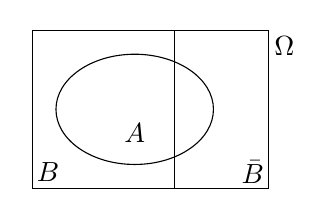
\begin{tikzpicture}
			\draw (0,0) rectangle (3,2);
			\draw (1.8,0) -- (1.8,2);
			\draw (1.3,1.0) ellipse (1.0cm and 0.7cm);
			\draw (0.2,0.2) node {$B$};
			\draw (2.8,0.2) node {$\bar{B}$};
			\draw (1.3,0.7) node {$A$};
			\draw (3.2,1.8) node {$\Omega$};
		\end{tikzpicture}
	\end{center}
\end{shaded}
Für eine Beobachtung \(a_1, \dots, a_n\) eines HMM suchen wir \(P(A_1=a_1, \dots, A_n=a_n)\).
Die Schwierigkeit dabei ist, dass die Zustandsfolge unbekannt ist.

Der naiver Ansatz ist die disjunkte Zerlegung nach Zustandsfolge \(Z_1, \dots, Z_n\):
\[P(A_1=a_1, \dots, A_n=a_n) = \sum\limits_{z_1, \dots, z_n} P(A_1=a_1, \dots, A_n=a_n, Z_1=z_1, \dots, Z_n=z_n)\]
Da diese Summe aus \(|Z|^n\) Summanden besteht, ist dies jedoch ineffizient.
Die Laufzeit wäre: $O(|Z|^n\cdot n)$.

Mit dynamischer Programmiereung berechnen wir
\begin{eqnarray}
	\alpha_t(j) &=& P(A_1=a_1, \dots, A_t=a_t,Z_t=j)\nonumber\\
				&=& \sum_i P(A_1=a_1, \dots, A_t=a_t, Z_{t-1}=i, Z_t=j)		\nonumber\\
				&=& \sum_i P(A_t=a_t|A_1=a_1, \dots, _{t-1}=a_{t-1}, Z_{t-1}=i,Z_t=j) \nonumber\\
				&& \cdot P(A_1=a_1, \dots, A_{t-1}=a_{t-1}, Z_{t-1}=i, Z_t=j)\nonumber\\
		&=& \sum_i P(A_t=a_t|Z_t=j) \cdot P(A_1=a_1,\dots, A_{t-1}=a_{t-1},Z_{t-1}=i,Z_t=j)\nonumber\\
				&=& \sum_i q_j(a_t) \cdot P(Z_t=j|Z_{t-1}=i) \cdot P(A_1=a_1, \cdots, A_{t-1}=a_{t-1}, Z_{t-1}=i)\nonumber\\
				&=& \sum_i q_j(a_t) \cdot p(i,j) \cdot \alpha_{t-1}(i)
				\label{eq:Forward_1}
\end{eqnarray}
\begin{figure}[htbp]
	\centering
	\begin{tikzpicture}[node distance=1.5cm]
		\node[state] (j)                 {j};
		\node[state] (i) [left=2cm of j]	{i};
        \node[state] (s1) [above=of i]	{};
		\node[state] (s2) [below=of i]	{};
		\node (at-1) [below =.5cm of s2] {\(a_{t-1}\)};
        \node (dots) [left=of at-1] {\(\dots\)};
        \node (a1) [left=of dots] {$a_1$};
		%\node[emission] (at) [below of=j] {\(a_t\)};
        \node[emission] (at) [right = 1.85cm of at-1] {\(a_t\)};
        \path[->]
			(s1) edge (j)
			(s2) edge (j)
			(i) edge [above] node {\(p(i,j)\)} (j)
			(j)	edge [right] node {\(q_j(a_t)\)} (at);
	\end{tikzpicture}
	\caption{Skizze des Forward-Algorithmus}
\end{figure}

Für t=1 gilt
\begin{equation}
	\alpha_1(j)=P(A_1=a_1, Z_1=j)=q_j(a_1)\cdot \pi_j
	\label{eq:Forward_2}
\end{equation}
Ferner gilt
\begin{eqnarray}
	P(A_1=a_1, \dots,A_n=a_n)	&=&\sum P(A_1=a_1, \dots, A_n=a_n, Z_n=j) \nonumber\\
								&=& \sum_j \alpha_n (j)
	\label{eq:Forward_3}
\end{eqnarray}
Mit (\ref{eq:Forward_1}), (\ref{eq:Forward_2}), (\ref{eq:Forward_3}) lässt sich die Wahrscheinlichkeit der Beobachtung \(a_1, \dots, a_n\) berechnen.
Aufwand dazu \(\underbrace{\mathcal{O}(n\cdot|Z|)}_{\text{Tabellengröße}}\cdot\underbrace{\mathcal{O}(|Z|)}_{\text{Aufwand pro Zelle}}+\underbrace{\mathcal{O}(|Z|)}_{\text{Aufsummierung}}=\mathcal{O}(n\cdot|Z|^2)\)



\section{Backward-Algorithmus}
Gegeben eine Beobachtung \(a_1, \dots, a_n\), was ist der wahrscheinlichste Zustand in Schritt \(t\)?
Gesucht ist also ein \(j\) mit \[P(Z_t=j|A_1=a_1, \dots, A_n=a_n)\] maximal.

Ansatz:
\begin{eqnarray*}
	&& P(A_1=a_1, \dots, A_n=a_n,Z_t=j)\\
	&=& P(A_{t+1}=a_{t+1}, \dots, A_n=a_n|A_1=a_1, \dots, A_t=a_t, Z_t=j)\\
	&&\cdot P(A_1=a_1, \dots, A_t=a_t,Z_t=j)\\
	&=& P(A_{t+1}=a_{t+1}, \dots, A_n=a_n|Z_t=j)\cdot P(A_1=a_1,\dots, A_t=a_t, Z_t=j)\\
	&=& \beta_t(j)\cdot\alpha_t(j)
\end{eqnarray*}
Ferner sei \(\beta_n(j)=1\) für alle \(j\).
Ähnlich wie in Forward-Algorithmus folgt:
\[\beta_t(j)=\sum_i p(j,i)\cdot q_i(a_{t+1}) \cdot \beta_{t+1}(i)\]

\begin{figure}[htbp]
	\centering
	\begin{tikzpicture}[node distance=1.5cm]
		\node[state] (j)				{\(j\)};
		\node[state] (s1)	[right of=j]	{};
		\node[state] (s2)	[above of=s1]	{};
		\node[state] (i)	[below of=s1]	{\(i\)};
		\node[emission] (at+1)	[below of=i]	{\(a_{t+1}\)};
		\node[emission] (at)	[left of=at+1]	{\(a_{t}\)};
		\node (...)				[right of=at+1]	{\(\dots\)};
		\node[emission]	(...)	[right of=...]	{\(a_n\)};
		\path[->] 
			(j) edge (s1)
			(j) edge (s2)
			(j) edge (i)
			(j) edge [right] node {\(p(j,i)\)} (i)
			(i)	edge [right] node {\(q_i(a_{t+1})\)} (at+1);
	\end{tikzpicture}
	\caption{Skizze des Backward-Algorithmuses}
\end{figure}

Die Laufzeit des Backward-Algorithmus liegt damit in 
\begin{align*}
    O(n\cdot{|Z|}^2).
\end{align*}

Die Wahrscheinlichkeit für den Zustand \(j\) im Schritt \(t\) ergibt sich aus
\begin{align*}
    P(Z_t=j|A_1=a_1, \dots, A_n=a_n) =&
    \frac{P(A_1=a_1,\ldots,A_n=a_n,Z_t=j)}{P(A_1=a_1,\ldots,A_n=a_n)}\\
=&\frac{\alpha_t(j)\cdot\beta_t(j)}{\sum_i \alpha_n(i)}
\end{align*}
Aufwand dazu \(\underbrace{\mathcal{O}(n\cdot|Z|^2)}_{\alpha\text{-Tabelle}} + \underbrace{\mathcal{O}(n\cdot|Z|^2)}_{\beta\text{-Tabelle}} + \underbrace{\mathcal{O}(|Z|)}_{\text{Summe}}+\underbrace{\mathcal{O}(1)}_{\text{Zugriff auf }\alpha_t(j) \text{und }\beta_t(j)}=\mathcal{O}(n\cdot|Z|^2)\)

\section{Posterior Decoding}
Wenn der Viterbi-Algorithmus viele unterschiedliche Pfade mit annähernd gleicher Wahrscheinlichkeit liefert, dann lässt sich die Wahl des wahrscheinlichsten Pfades nicht gut rechtfertigen.
Alternativ können wir mit dem Backward-Algorithmus die Folge der in jedem
Zeitpunkt $t$ wahrscheinlichsten Zustände
\[ \hat z_{t} = \arg_{j}\max P(Z_{t} = j | A_{1} = a_{1}, \ldots, A_{n} = a_{n}) \]
bestimmen.
Diese muss jedoch keine zuverlässige Folge sein.

\begin{shaded}
\paragraph{Übung}
\label{par:ubung}

Es sollen codierende und nicht-codierende Abschnitte in DNA bestimmt werden.
Vorhanden sind:
\begin{itemize}
    \item einige codierende Sequenzen
    \item einige nicht-codierende Sequenzen
    \item große Menge an unbekannten Sequenzen
\end{itemize}
Gesucht ist ein Verfahren um codierende Regionen in DNA zu identifizieren,
gegeben eine DNA Sequenz.\\
Lösung:
\begin{itemize}
    \item Hidden-Markov-Model wie in BildX
    \item jeweils einen ML-Schäter für beide Zustandsmenge \{codierend,
        nicht-codierend\} (überwachtes Training)
    \item Übergangswahrscheinlichkeiten zwischen den Zustandsmengen \{codierend,
        nicht-codierend\} mittels unüberwachtem Training (Viterbi-Training oder
        Baum-Welch-Algorithmus)
    \item Backward-Algorithmus
        \begin{align*}
            P(Z_t \in \{a_c,c_c,g_c,t_c\} | A_1=a_1,\ldots,A_n=a_n)=\\
            \sum\limits_{z\in a_c,c_c,g_c,t_c} P(Z_t=z|A_1=a_1,\ldots,A_n=a_n)
        \end{align*}
\end{itemize}
Wenn das Ergebnis größer als $\frac{1}{2}$ ist, ist es eine codierende Sequenz,
sonst uncodierend.
\end{shaded}

\begin{shaded}
\paragraph{Übung}
\label{par:ubung2}

Gegeben sei ein HMM.
In diesem werden die Zustände verdoppelt.
Wie muss sich die Länge der Trainigssequenz erhöhen, damit die gleiche Anzahl Zustandsübergänge vorhanden ist wie vorher.
Vereinfacht sein angenohmen das alle Zustandsübergänge die gleiche Wahrscheinlichkeiten besitzen.

Lösung:
\[\hat p(z,z') = \frac{n}{|z^2|}\]
Die Trainigssequenz muss 4-fach solang sein.
\end{shaded}

\section{Baum-Welch-Algorithmus}
Der Baum-Welch-Algorithmus wird benutzt, um die unbekannten Parameter eines Hidden Markov Models (HMM) zu finden.
Er nutzt dabei den Forward-Backward-Algorithmus zur Berechnung von Zwischenergebnissen, ist aber nicht mit diesem identisch.
Der Baum-Welch-Algorithmus ist ein erwartungsmaximierender Algorithmus.

Idee:
\begin{enumerate}
	\item HMM zufällig initialisieren
	\item Mit dem Backward-Algorithmus die Wahrscheinlickeit \[P(Z_{t} = j \| A_{1} = a_{1}, \ldots, A_{n} = a_{n})\]berechnen.
			Auf ähnliche Weise lassen sich \[P(Z_{t} = i, Z_{t+1} = j \| A_{1} = a_{1}, \ldots, A_{n} = a_{n})\] berechnen.
			Damit lassen sich Erwartungswerte berechen für die Häufigkeit eines Zustandes, eines Zustandsübergangs oder einer Emission.
			Damit lassen sich Schätzer berechnen für die Parameter des HMM.
			Damit werden die Parameter des HMM geändert.
	\item Mehrfach iterieren, bis sich an den Parametern nichts mehr ändert, beste Lösung ausgeben (größte Wahrscheinlichkeit für Ausgabesequenz)
\end{enumerate}
